\NeedsTeXFormat{LaTeX2e}
\documentclass{jfp}

\title{Composing data visualizations}
\author[Tomas Petricek]{TOMAS PETRICEK\\
       University of Kent, UK\\
       \email{t.petricek@kent.ac.uk}}

\begin{document}
\maketitle[f]

% \begin{abstract}
% This guide is for authors who are preparing papers for the \emph{Journal of
% Functional Programming} using the \LaTeXe\ document-preparation system
% and the Functional Programming class file (\texttt{jfp1.cls}).
% \end{abstract}


\bibliographystyle{jfp}

\section{Introduction}
Let's say we want to create the two charts in Figure~\ref{fig:charts}. The chart on the left is
a bar chart, except that it shows two different values for each bar. The chart on the
right is a line chart, except that it also highlights two parts of the timeline with two different
colors.

There is a plenty of libraries that can draw bar charts and line charts, but adding those extra
features will only be possible if the author already thought about your exact scenario. For
example, Google Charts supports the left chart (it is called Dual-X Bar Chart) but there is no
way for adding a background, let alone based on the X value. The alternative is to use a more
low-level library such as D3. In D3 you construct the chart piece by piece, but then you have to
tediously transform your values to coordinates in pixels. For scientific data visualizations,
you could use an implementation of the Grammar of Graphics such as ggplot2. This lets you
map data to geometric objects (such as points, bars, and lines) and their visual properties
(X and Y coordinate, shape and color). However, the number of options is still somewhat limited.

To a functional programmer, this situation is disappointing. We should be able to
compose a variety of charts from a small number of primitives. The shapes should be defined
not in terms of pixels, but numbers of seats or exchange rates. We should also be able to easily
derive high-level abstractions, such as a bar chart, from those low-level primitives.

\begin{figure}
  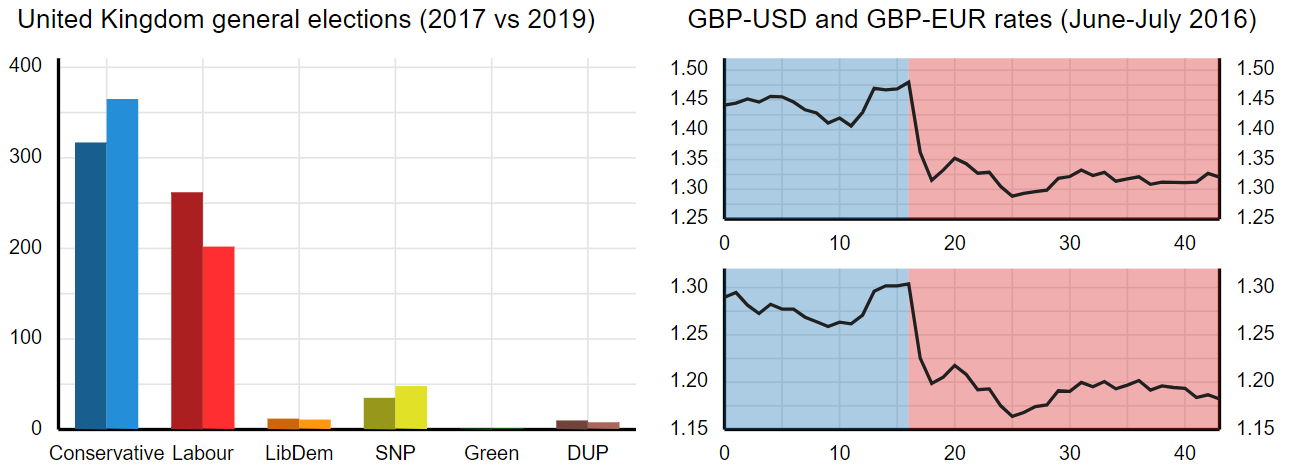
\includegraphics[scale=0.57]{figures/charts}
  \vspace{0.25em}
  \caption{Two charts about the UK politics: Comparison of election results from 2017 and 2019 (left)
    and GBP-USD exchange rate with highlighted areas before and after the 23 June 2016 Brexit vote.}
  \label{fig:charts}
\end{figure}

In this paper, we...

\newpage


\section{Domain specific language}
\label{sec:intro}
\subsection*{Domain-specific values}


All values that are provided when constructing charts are from the chart domain. For example,
when visualizing the population of different countries, X values will be categorical values
such as \strf{United Kingdom} or \strf{Czech Republic} and Y values will be continuous values
such as $\num{66.04}$ million or $\num{10.58}$ million. Compost will automatically map the value
from a domain value to a pixel value. The user does not need to do any rescaling to obtain
value in pixels. This is akin to most high-level charting libraries, but in contrast with some
more flexible libraries like, say, D3.
Compost supports only two-dimensional charts and values can be either categorical (such as
different countries) or continuous (such as population size). A value needs to determine an
exact position in the space available for the chart. For continuous values, this simply means
applying a linear transformation. For categorical values, the situation is more difficult. For % example,
say we are drawing a bar chart with population of three different countries with countries
on the X axis and population on the Y axis. The scale of the X axis is categorical and
Compost divides the available space into three ranges of equal width. However, then \strf{United % Kingdom}
or \strf{Czech Republic} does not determine an exact position but instead a range. To determine
a unique position, we need to attach a value between $\num{0}$ and $\num{1}$ to the
categorical value which identifies a relative position in the available range. This is
illustrated in Figure~\ref{fig:scales}.
\begin{figure}[!h]
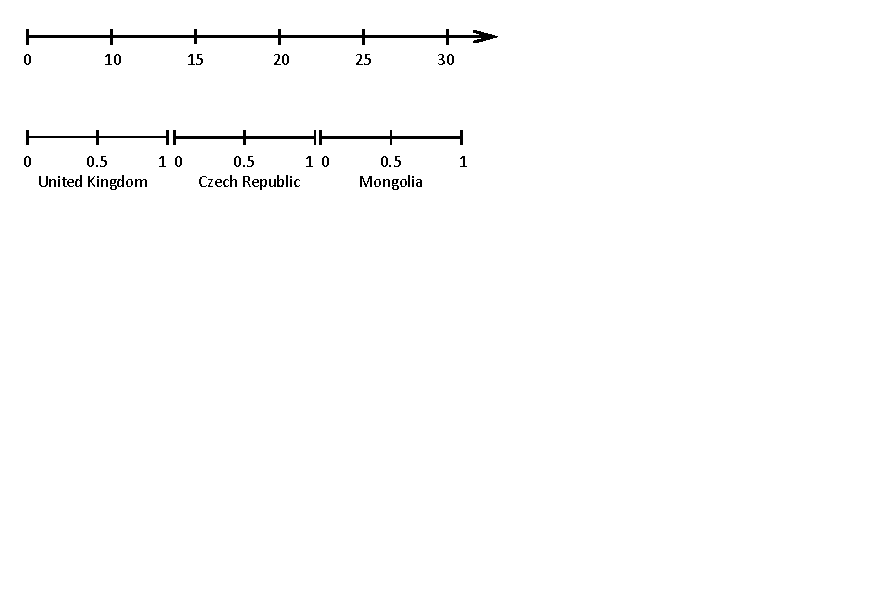
\includegraphics[scale=1,trim={0cm 6.5cm 6cm 0cm},clip]{values.pdf}
\caption{Values on a continous scale and categorical scale.}
\label{fig:scales}
\end{figure}
More formally, we write $c$ for categorical values such as countries (represented as country
names using strings), $r$ for ratio between $0$ and $1$ and we write $n$ for numerical continuous
values with any range. A value $v$ used in a Compost chart is defined as:
%
\begin{equation*}
\begin{array}{rcl}
v & = & \kvd{cat}~c, r \lsep \kvd{cont}~n
\end{array}
\end{equation*}
%
A value $v$ that is used to create Compost charts can be categorical, written as \kvd{cat} and
consisting of the category and a ratio that determines point in the space allocated for the
cateogry. A continous value, written as \kvd{cont}, consists of a number and will be mapped to
a location based on the implicitly obtained re-scaling.
\subsection*{Language of composable charts}
Now that we defined our representation of values, we can define a basic composable language of
data visualizations. A shape $s$ represents a chart. In the most basic form, it can be text label,
line connecting a list of points and a filled polygon determined by a list of points. For line,
text and polygon, we also include a parameter $\gamma$ indicating the color to be used. In addition,
a shape can be constructed by overlaying several other shapes:
%
\begin{equation*}
\begin{array}{rcl}
s & = & \kvd{overlay}~s_1, \ldots, s_n\\
 & | & \kvd{text}~\gamma, v_x, v_y, t\\
 & | & \kvd{line}~\gamma, v_{x1}, v_{y1}, \ldots, v_{xn}, v_{yn}\\
 & | & \kvd{fill}~\gamma, v_{x1}, v_{y1}, \ldots, v_{xn}, v_{yn}
\end{array}
\end{equation*}
%
As an example, consider bar chart with \strf{UK} and \strf{CZ} as two categorical values on the X
axis and their population in millions (continuous value) on the Y axis. This can be constructed by
creating two filled rectangles using \kvd{fill} and overlaying them using \kvd{overlay}:
%
\begin{equation*}
\begin{array}{l}
\kvd{overlay}\\
\quad \kvd{fill}~\strf{\#0000ff},
 ~(\kvd{cat}~\strf{UK}, \num{0}), (\kvd{cont}~\num{00.00}), (\kvd{cat}~\strf{UK}, \num{0}), % (\kvd{cont}~\num{66.04}),\\
\hspace{5.9em}(\kvd{cat}~\strf{UK}, \num{1}), (\kvd{cont}~\num{66.04}), (\kvd{cat}~\strf{UK}, % \num{1}), (\kvd{cont}~\num{00.00}),\\
\quad \kvd{fill}~\strf{\#ff0000},
 ~(\kvd{cat}~\strf{CZ}, \num{0}), (\kvd{cont}~\num{00.00}), (\kvd{cat}~\strf{CZ}, \num{0}), % (\kvd{cont}~\num{10.58}),\\
\hspace{5.9em}(\kvd{cat}~\strf{CZ}, \num{1}), (\kvd{cont}~\num{10.58}), (\kvd{cat}~\strf{CZ}, % \num{1}), (\kvd{cont}~\num{00.00})\\
\end{array}
\end{equation*}
%
The shape specification overlays two bars of different colours. To construct a rectangle, we
define four points. For the UK, two of the points have Y value set to 0 (bottom of the bar) and
two have it set to 66.04 (top of the bar indiciating the population value). The values on the X
axis are categorical \strf{UK} values -- two are on the left as indicated by the ratio $\num{0}$
and two are on the right as indicated by ratio $\num{1}$. The ratio is always relative to the
category, so the ratios for the second bar are also $\num{0}$ and $\num{1}$.
\subsection*{Calculating scales and projections}
When processing shape specification such as the one given in the previous section, the Compost
library infers the scales for the X and Y axes and computes a projection function that can be
used for mapping domain-specific values to pixels. While doing this, it also checks for consistency % --
all values on one axis have to be either categorical or continuous, but not a mix of the two.
The first step is to determine the scales for each of the axes. A scale can be continuous,
defined by a minimal and maximal value, or a categorical, defined by a list of categorical values.
Note that we do not need to track the ratios used as each category
will be allocated equal amount of space, regardless of where in that space shapes need to
appear. A scale $l$ is thus defined as:
%
\begin{equation*}
\begin{array}{rcl}
l & = & \kvd{categorical}~c_1, \ldots, c_k \lsep \kvd{continuous}~n_{min}, \ldots, n_{max}
\end{array}
\end{equation*}
%
A scale is obtained by recursively walking over the shape and gradually constructing two scales,
for X and Y axis, from the X and Y coordinates that appear in the shape. The process is fairly
straightforward and we won't discuss it in detail (for now). The first value encountered determines
what kind of a scale will be constructed. If the type of a later value does not match the type of a
scale, the process fails.
Once we obtain scales for both X and Y axes, we calculate a projection function for each axis.
The function takes a value $v$ together with total space available (say, in pixels) and produces
a position in pixels corresponding to $v$. We also omit the details here (for now), but briefly --
for continuous values, we produce a simple linear transformation; for categorical values, we split
the available space into $k$ equally sized regions (where $k$ is the number of categorical values
in the scale) and then map a categorical value $\kvd{cat}~c, r$ to the region corresponding to $c$
according to the ratio $r$.
\subsection*{Controlling and nesting scales}
The process of computing scales can be controlled by additional primitives in the Compost
domain-specific language for describing shapes that were not discussed earlier. The following
definition lists additional primitives that are also a part of the definition of $s$. Note that
the primitives can be applied either to the X scale or to the Y scale - we write $x/y$ to indicate
that a sub-script on those primitives can be set either to $x$ or to $y$ (both scales can be
modified by nesting two primitives):
%
\begin{equation*}
\begin{array}{rcl}
s & = & (\ldots)\\
 & | & \kvd{axis}_{x/y} s\\
 & | & \kvd{roundScale}_{x/y} s\\
 & | & \kvd{explicitScale}_{x/y}~l, s\\
 & | & \kvd{nest}_{x/y}~v_{min}, v_{max}, s
\end{array}
\end{equation*}
%
We first focus on the first three primitives, while the \kvd{nest} primitive will be discussed in
the next section. The \kvd{axis} and \kvd{roundScale} constructs could be defined as derived % constructs,
but it is easier to consider them as primitives for now. The \kvd{axis} primitive simply takes the % shape
$s$ and draws an axis around the contents of $s$, using the inferred scale of $s$ to determine % values
displayed on the axis. This could be a derived construct, because axes can be rendered using lines
and text labels.
The \kvd{roundScale} operation takes the inferred X or Y scale of the shape $s$ and, if it is a
continuous scale, rounds its minimal and maximal values to ``nice'' numbers. For example, if a
continuous scale has minimum $\num{0}$ and maximum $\num{66.04}$, the resulting scale would have
maximum $\num{70}$. For categorical scale, the operation does not have any effect.
The \kvd{explicitScale} operation is similar, but it replaces the inferred scale with an explicitly
provided scale (the type of the inferred scale has to match with the type of the explicitly given
scale). For example, assuming \ident{populationBar} is the example given earlier, we can write:
%
\begin{equation*}
\begin{array}{l}
\kvd{axis}_x~(\kvd{axis}_y~(\kvd{roundScale}_y\\
\quad(\kvd{explicitScale}_x~(\kvd{categorical % \strf{CZ},\strf{MN},\strf{UK}})~\ident{populationBar})))
\end{array}
\end{equation*}
%
This replaces the X axis with an explicitly given one that includes extra country code and also
overrides the implicitly inferred order of the categorical values. We then ask Compost to
automatically round the Y scale (showing population) so that we get a ``nice'' number as the
maximum. Finally, we add axes around the shape, producing a usual labelled chart.
As noted earlier, both \kvd{axis} and \kvd{roundScale} could be defined as derived -- \kvd{axis}
would have to infer the scales of the nested shape, calculate appropriate labels and insert
suitable lines and labels; the \kvd{roundScale} operation would need to infer the scale too and
then add an explicit \kvd{explicitScale} with a rounded minimal and maximal value of a continuous
scale.
\begin{figure}[!h]
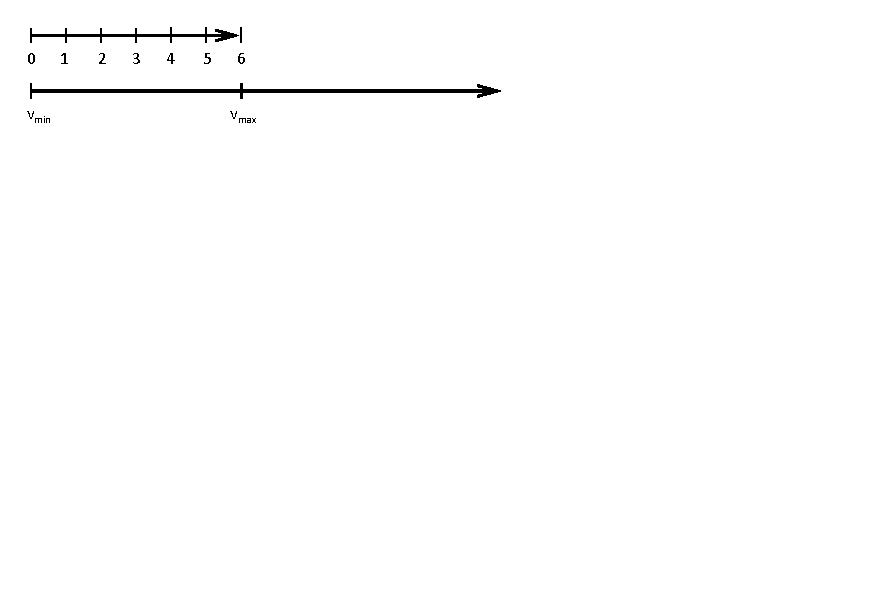
\includegraphics[scale=1,trim={0cm 7.5cm 6cm 0cm},clip]{nest.pdf}
\caption{A continuous scale with values from $0$ to $6$, nested in another scale.}
\label{fig:nesting}
\end{figure}
\subsection*{Nesting of charts and scales}
Finally, one more primitive that we added in the above definition and that we have not explained
yet is $\kvd{nest}_{x/y}$. The parameters of the primitive are two values, $v_{min}$ and $v_{max}$
together with a shape $s$. The primitive makes it possible to nest one scale inside another
one.
When inferring the scales, Compost infers the scale of the nested shape $s$. This will then take
the area determined by the two points $v_{min}$ and $v_{max}$ in the scale determined by other
shapes that are overlaid with the $\kvd{nest}$ shape. The two points are also used to determine
the scales of the overall shape, but the scales of $s$ are nested and do not have any effect on
the outer scales. In fact, the scale of $s$ does not even have to be of the same type as the
scale of the outer shape.
Figure~\ref{fig:nesting} illustrates this with an example. Here, we are nesting a continuous scale
with values ranging from $\num{0}$ to $\num{6}$ into another scale. The values $v_{max}$ and
$v_{min}$ do not even have to be continuous. We can, for example, nest a line chart inside a
bar of a bar chart and then the two values could be $\kvd{cat}~\strf{One}, 0$ and % $\kvd{cat}~\strf{One}, 1$
(which are two values that define a region of a categorical scale).
One area where nesting of scales is particularly useful is when combining multiple charts in
a single view. For example, let's say that we have two line charts showing prices of two different
stocks over the same period of time (for simplicity, we can just use UNIX timestamp as a time).
The prices of the two stocks are orders of magnitude different, so they cannot fit easily into the
same chart. We want to show two line charts side-by-side (one above each other). They should each
have their own Y axis (price), but the X axis (time) should be shared.
Assuming we have \ident{googPrices} and \ident{fbPrices} as two line charts without any axes,
covering the same date range, we can write:
%
\begin{equation*}
\begin{array}{l}
\kvd{axis}_x~(\kvd{overlay}\\
\quad (\kvd{nest}_y~(\kvd{cat}~\strf{top-chart}, \num{0}), (\kvd{cat}~\strf{top-chart}, \num{1}),
 (\kvd{axis}_y~\ident{fbPrices})),\\
\quad (\kvd{nest}_y~(\kvd{cat}~\strf{bottom-chart}, \num{0}), (\kvd{cat}~\strf{bottom-chart}, % \num{1}),
 (\kvd{axis}_y~\ident{googPrices}))~)\\
\end{array}
\end{equation*}
%
Reading the code from the inner-most part to the outer-most, we first add separate Y axes to both
of the line charts. Given the difference in the prices, the axes will have quite different values.
We then nest the (continuous) Y axes using the \kvd{nest} primitive and, at the same time, % implicitly
define a new outer Y axis. The outer Y axis is categorical with just two values, \strf{top-chart}
and \strf{bottom-chart}. This means that the two nested charts will take equal amount of space,
one above the other (each of the charts takes the full space allocated for the category -- the
minimal value has ratio $0$ while the maximal value has ratio $1$).
~
~
\noindent
[TODO: We really need illustrations for those example charts, but that would be more work!]
~
[TODO: Maybe use this chart as a motivation: https://wellcomeopenresearch.org/articles/4-63/v1]
~
\section{Random ideas}
\begin{itemize}
\item We could define a type system to catch categorical/continuous value mismatch in a single % scale.
\item It would be worth thinking about ordinal values, which are categorical but can be sorted.
\item There might be other kinds of scales - for example, color scale (can have meaning in scatter % plot)
 or a scale for secondary markers (like sizes of bubbles in a bubble chart). We could really say % that
 every value (including bar chart colors) should be coming from some scale...
\item Implementing something like \kvd{axis} or \kvd{roundScale} as an actual derived primitive is
 a bit tricky, because it needs to invoke a part of the normal rendering workflow (to run the
 automatic inference of scales on the nested shape) -- this might be just implementation issue,
 but it could be some more basic problem.
\end{itemize}
\end{document}

%


% \usepackage{booktabs}
% \usepackage{subcaption}
% \usepackage{lineno,hyperref,xcolor}
% \usepackage{flushend}
% \usepackage{stmaryrd}
% \usepackage{amssymb}
% \usepackage{xypic}
% \usepackage{semantic}
% \usepackage{booktabs}
% \usepackage{enumitem}
% \usepackage{enumerate}
% \usepackage{amsmath}
% \usepackage[T1]{fontenc}
%
% \setlist{leftmargin=6mm}
% \newcounter{thc}
% \newcounter{dfc}
%
% \theoremstyle{plain}
% \newtheorem{lem}[thc]{Lemma}
% \newtheorem{theorem}[thc]{Theorem}
%
% \theoremstyle{definition}
% \newtheorem{axiom}[dfc]{Axiom}
% \newtheorem{definition}[dfc]{Definition}
%
% \title{Compost: Library for composable data visualization}
% %\author{Tomas Petricek}
% %\affiliation{
% %  \institution{University of Kent}
% %  \country{United Kingdom}
% %}
% %\email{tomas@tomasp.net}
%
% %\begin{CCSXML}
% %<ccs2012>
% %<concept>
% %<concept_id>10011007.10011006.10011008</concept_id>
% %<concept_desc>Software and its engineering~General programming languages</concept_desc>
% %<concept_significance>500</concept_significance>
% %</concept>
% %<concept>
% %<concept_id>10003456.10003457.10003521.10003525</concept_id>
% %<concept_desc>Social and professional topics~History of programming languages</concept_desc>
% %<concept_significance>300</concept_significance>
% %</concept>
% %</ccs2012>
% %\end{CCSXML}
% %
% %\ccsdesc[500]{Software and its engineering~General programming languages}
% %\ccsdesc[300]{Social and professional topics~History of programming languages}
%
% \definecolor{cmtclr}{rgb}{0.0,0.6,0.0}
% \definecolor{kvdclr}{rgb}{0.0,0.0,0.6}
% \definecolor{idclr}{rgb}{0.0,0.0,0.0}
% \definecolor{numclr}{rgb}{0.0,0.4,0.0}
% \definecolor{strclr}{rgb}{0.4,0.4,0.0}
% \definecolor{rstrclr}{rgb}{0.5,0.1,0.0}
% \definecolor{prepclr}{rgb}{0.6,0.0,0.2}
% \newcommand{\vect}[1]{\langl #1 \rangl}
% \newcommand{\langl}{\begin{picture}(4.5,7)
% \put(1.1,2.5){\rotatebox{60}{\line(1,0){5.5}}}
% \put(1.1,2.5){\rotatebox{300}{\line(1,0){5.5}}}
% \end{picture}}
% \newcommand{\rangl}{\begin{picture}(4.5,7)
% \put(.9,2.5){\rotatebox{120}{\line(1,0){5.5}}}
% \put(.9,2.5){\rotatebox{240}{\line(1,0){5.5}}}
% \end{picture}}
% \newcommand{\ball}[1]{\FPeval{\result}{clip(201+#1)}\textnormal{\ding{\result}}}
% \newcommand{\lsep}{\;\;|\;\;}
% \newcommand{\num}[1]{\textcolor{numclr}{#1}}
% \newcommand{\str}[1]{\textnormal{\textcolor{strclr}{\sffamily "#1"}}}
% \newcommand{\strf}[1]{\textnormal{\textcolor{strclr}{\sffamily #1}}}
% \newcommand{\rstr}[1]{\textnormal{\textcolor{rstrclr}{\sffamily "#1"}}}
% \newcommand{\ident}[1]{\textnormal{\textcolor{idclr}{\sffamily #1}}}
% \newcommand{\qident}[1]{\textnormal{\sffamily \textquotesingle #1\textquotesingle}}
% \newcommand{\dom}{\ident{dom}}
% \newcommand{\kvd}[1]{\textnormal{\textcolor{kvdclr}{\sffamily #1}}}
%
% \newcommand{\bndclr}[1]{\textcolor{kvdclr}{#1}}
% \newcommand{\bkndclr}[1]{\textcolor{prepclr}{#1}}
% \newcommand{\blblclr}[1]{\textcolor{numclr}{#1}}
% \newcommand{\bnd}[1]{\textnormal{\textcolor{kvdclr}{\sffamily #1}}}
% \newcommand{\bknd}[1]{\textnormal{\textcolor{prepclr}{\sffamily #1}}}
% \newcommand{\blbl}[1]{\textnormal{\textcolor{numclr}{\sffamily #1}}}
% \newcommand{\narrow}[1]{\hspace{-0.6em}#1\hspace{-0.6em}}
% \newcommand{\rname}[1]{{\sffamily\small(#1)}}
% \newcommand{\ername}[1]{\vspace{0.75em}\rname{#1}\hspace{0.5em}}
% \newcommand{\preview}[1]{\,\textnormal{\guillemotleft} #1\textnormal{\guillemotright}\,}
%
% \begin{document}
% %\begin{abstract}
% %\end{abstract}
% \maketitle
%
% % ==================================================================================================
%
